\documentclass[9pt]{beamer}

\usetheme{Madrid}

\usepackage{hyperref}

\usepackage{tikz}

\usetikzlibrary{arrows.meta,positioning}

% 设置全局字号

\setbeamerfont{normal text}{size=\scriptsize}

\setbeamerfont{title}{size=\Large}

\setbeamerfont{frame title}{size=\normalsize}

\setbeamerfont{block title}{size=\small}

\setbeamerfont{itemize/enumerate body}{size=\footnotesize}

% 减少列表间距

\setlength{\itemsep}{2pt}

\setlength{\parsep}{1pt}

% 为所有frame设置更紧凑的布局

\setbeamersize{text margin left=0.5cm,text margin right=0.5cm}

% 设置块内容字号

\setbeamerfont{block body}{size=\footnotesize}

\title{Progress Report\\\vspace{0.3em}Interface Fuzzing for Isabelle/Sledgehammer}

\subtitle{Knowledge Exchange Projects - Amazon — Variant 3}

\author{Qilan Lin (K21204786)}

\institute{King's College London}

\date{10\textsuperscript{th} December 2025}

\begin{document}

%------------------------------------------------

% Slide 1: Title

%------------------------------------------------

\begin{frame}

  \titlepage

  \vspace{-0.5cm}

  \begin{center}

  \textbf{Project Description:} Fuzzing the interface between Isabelle/HOL's Sledgehammer and external ATP/SMT provers to improve reliability and discover integration bugs.

  \end{center}

\end{frame}

%------------------------------------------------

% Slide 2: Current State (What you have achieved)

%------------------------------------------------

\begin{frame}{Current State of Project}

\begin{block}{Overall Progress: 85\% Complete — \textcolor{green}{On Track}}

\begin{center}

\scalebox{0.7}{

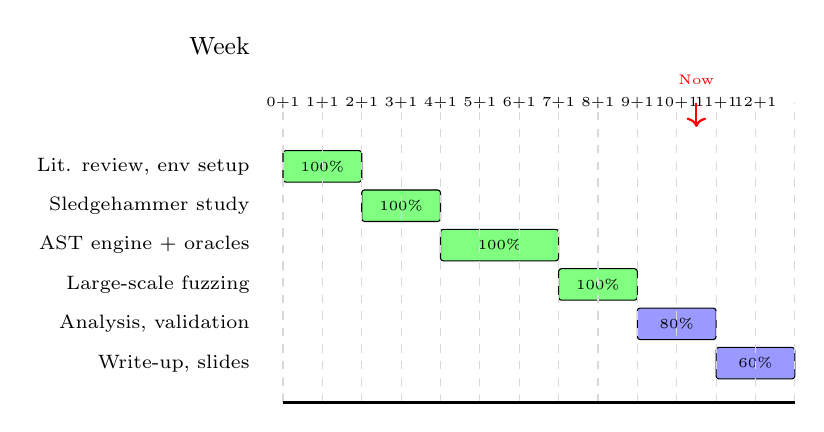
\begin{tikzpicture}[
    ganttbar/.style={draw, fill=blue!40, minimum height=0.5cm, rounded corners=1pt},
    ganttdone/.style={draw, fill=green!50, minimum height=0.5cm, rounded corners=1pt},
    ganttlabel/.style={anchor=east, font=\scriptsize},
    weeklabel/.style={font=\tiny, anchor=north}
]

    % Week labels (x-axis)

    \foreach \x in {0,...,12} {

        \node[weeklabel] at (\x*0.5, 5.5) {\x+1};

    }

    \node[anchor=south east, font=\small] at (-0.3, 5.8) {Week};

    

    % Task 1: Literature review, environment setup (Week 1-2) - DONE

    \node[ganttlabel] at (-0.3, 4.5) {\scriptsize Lit. review, env setup};

    \draw[ganttdone] (0, 4.3) rectangle (1, 4.7);

    \node[font=\tiny] at (0.5, 4.5) {100\%};

    

    % Task 2: Sledgehammer study (Week 3-4) - DONE

    \node[ganttlabel] at (-0.3, 4.0) {\scriptsize Sledgehammer study};

    \draw[ganttdone] (1, 3.8) rectangle (2, 4.2);

    \node[font=\tiny] at (1.5, 4.0) {100\%};

    

    % Task 3: AST engine + oracles (Week 5-7) - DONE

    \node[ganttlabel] at (-0.3, 3.5) {\scriptsize AST engine + oracles};

    \draw[ganttdone] (2, 3.3) rectangle (3.5, 3.7);

    \node[font=\tiny] at (2.75, 3.5) {100\%};

    

    % Task 4: Large-scale fuzzing (Week 8-9) - DONE

    \node[ganttlabel] at (-0.3, 3.0) {\scriptsize Large-scale fuzzing};

    \draw[ganttdone] (3.5, 2.8) rectangle (4.5, 3.2);

    \node[font=\tiny] at (4, 3.0) {100\%};

    

    % Task 5: Minimization, analysis (Week 10-11) - IN PROGRESS

    \node[ganttlabel] at (-0.3, 2.5) {\scriptsize Analysis, validation};

    \draw[ganttbar] (4.5, 2.3) rectangle (5.5, 2.7);

    \node[font=\tiny] at (5, 2.5) {80\%};

    

    % Task 6: Write-up, slides (Week 12-13) - IN PROGRESS

    \node[ganttlabel] at (-0.3, 2.0) {\scriptsize Write-up, slides};

    \draw[ganttbar] (5.5, 1.8) rectangle (6.5, 2.2);

    \node[font=\tiny] at (6, 2.0) {60\%};

    

    % Grid lines

    \foreach \x in {0,...,13} {

        \draw[gray!30, dashed] (\x*0.5, 1.5) -- (\x*0.5, 5.3);

    }

    \draw[thick] (0, 1.5) -- (6.5, 1.5);
    
    % Current week indicator
    \draw[red, thick, ->] (5.25, 5.3) -- (5.25, 5.0);
    \node[font=\tiny, red] at (5.25, 5.6) {Now};

\end{tikzpicture}

}

\end{center}

\end{block}

\begin{block}{Major Achievements}

\begin{itemize}\footnotesize

  \item ✓ \textbf{AST-Based Fuzzer}: 10 mutation operators, 204 mutations tested, 8000+ LOC

  \item ✓ \textbf{Differential Testing}: 519 prover performance anomalies discovered

    \begin{itemize}\tiny

      \item E Prover: 349 (67.2\%), cvc5: 143 (27.6\%), Z3: 27 (5.2\%)

      \item Types: Timeouts (288), Errors (115), Slowdowns (116)

    \end{itemize}

  \item ✓ \textbf{Integration Testing}: 267 total tests, \textbf{0 integration bugs}

    \begin{itemize}\tiny

      \item 204 AST mutations + 63 aggressive reconstruction tests

      \item Mirabelle validation + hidden exception detection

    \end{itemize}

\end{itemize}

\end{block}

\end{frame}

%------------------------------------------------

% Slide 3: Key Results

%------------------------------------------------

\begin{frame}{Key Results \& Findings}

\begin{block}{Prover Performance Anomalies (519 Total)}

\begin{center}

\scalebox{0.85}{

\begin{tabular}{l|r|r|r|r}

\textbf{Prover} & \textbf{Timeout} & \textbf{Error} & \textbf{Slowdown} & \textbf{Total} \\

\hline

E Prover & 186 & 67 & 96 & 349 (67.2\%) \\

cvc5 & 83 & 41 & 19 & 143 (27.6\%) \\

Z3 & 19 & 7 & 1 & 27 (5.2\%) \\

\hline

\textbf{Total} & \textbf{288} & \textbf{115} & \textbf{116} & \textbf{519} \\

\end{tabular}

}

\end{center}

\end{block}

\begin{block}{Integration Layer Testing (267 Tests)}

\begin{itemize}\footnotesize

  \item ✓ \textbf{AST Mutations}: 204 mutations, 11 seed theories, 9/10 operators used

  \item ✓ \textbf{Aggressive Stress Tests}: 63 edge-case tests targeting reconstruction

    \begin{itemize}\tiny

      \item Type breaking, encoding attacks, extreme values, Unicode injection

      \item Boundary conditions, proof corruption, configuration fuzzing

    \end{itemize}

  \item ✓ \textbf{Result}: \textcolor{green}{\textbf{0 integration bugs}}, \textcolor{green}{\textbf{0 hidden exceptions}}, \textcolor{green}{\textbf{0 reconstruction bugs}}

\end{itemize}

\end{block}

\begin{block}{Key Insight}

\begin{center}

\textit{``Reliability issues are concentrated in external provers (519 anomalies),\\not in Sledgehammer's integration layer (0 bugs in 267 tests).''}

\end{center}

\end{block}

\end{frame}

%------------------------------------------------

% Slide 4: Remaining Work & Next Steps

%------------------------------------------------

\begin{frame}{Remaining Work \& Next Steps}

\begin{block}{Completed Tasks (\textcolor{green}{85\%})}

\begin{itemize}\footnotesize

  \item ✓ Literature review, environment setup (100\%)

  \item ✓ Sledgehammer study and analysis (100\%)

  \item ✓ AST mutation engine with 10 operators (100\%)

  \item ✓ Differential oracle for prover testing (100\%)

  \item ✓ Mirabelle integration for validation (100\%)

  \item ✓ Large-scale fuzzing campaigns (100\%)

  \item ✓ Hidden exception detection via instrumentation (100\%)

  \item ✓ Aggressive reconstruction stress testing (100\%)

\end{itemize}

\end{block}

\begin{block}{Remaining Tasks (\textcolor{orange}{15\%})}

\begin{itemize}\footnotesize

  \item \textbf{Paper finalization} (80\% done): Final proofreading, formatting

  \item \textbf{Code documentation}: README updates, usage examples

  \item \textbf{Final presentation}: Slides preparation

\end{itemize}

\end{block}

\begin{block}{Timeline}

\begin{itemize}\footnotesize

  \item \textbf{This week}: Complete paper draft, finalize all figures/tables

  \item \textbf{Next week}: Code cleanup, documentation, presentation prep

  \item \textbf{Final week}: Submission and presentation

\end{itemize}

\end{block}

\begin{center}

\textbf{Status: \textcolor{green}{On track for successful completion}}

\end{center}

\end{frame}

\end{document}

